\section{THIẾT KẾ HỆ THỐNG VÀ QUY HOẠCH}

\subsection{Sơ đồ Topology tổng thể}
Hệ thống mạng được thiết kế và xây dựng trên mô hình giả lập gồm một mạng lõi MPLS Backbone của nhà cung cấp dịch vụ (ISP) đứng ở vị trí trung tâm, chịu trách nhiệm kết nối 3 chi nhánh doanh nghiệp có khoảng cách xa nhau.

\begin{figure}[H]
    \centering
    % [NOTE] SAU KHI BUILD PDF, BẠN CẦN LƯU ẢNH SƠ ĐỒ MẠNG (ĐANG NẰM TRONG FOLDER IMAGE HOẶC VẼ LẠI) VÀO FOLDER image/ VỚI TÊN network_topology.png. KHÔNG CẦN BỎ COMMENT DÒNG DƯỚI VÌ NÓ ĐÃ UNCOMMENTED.
    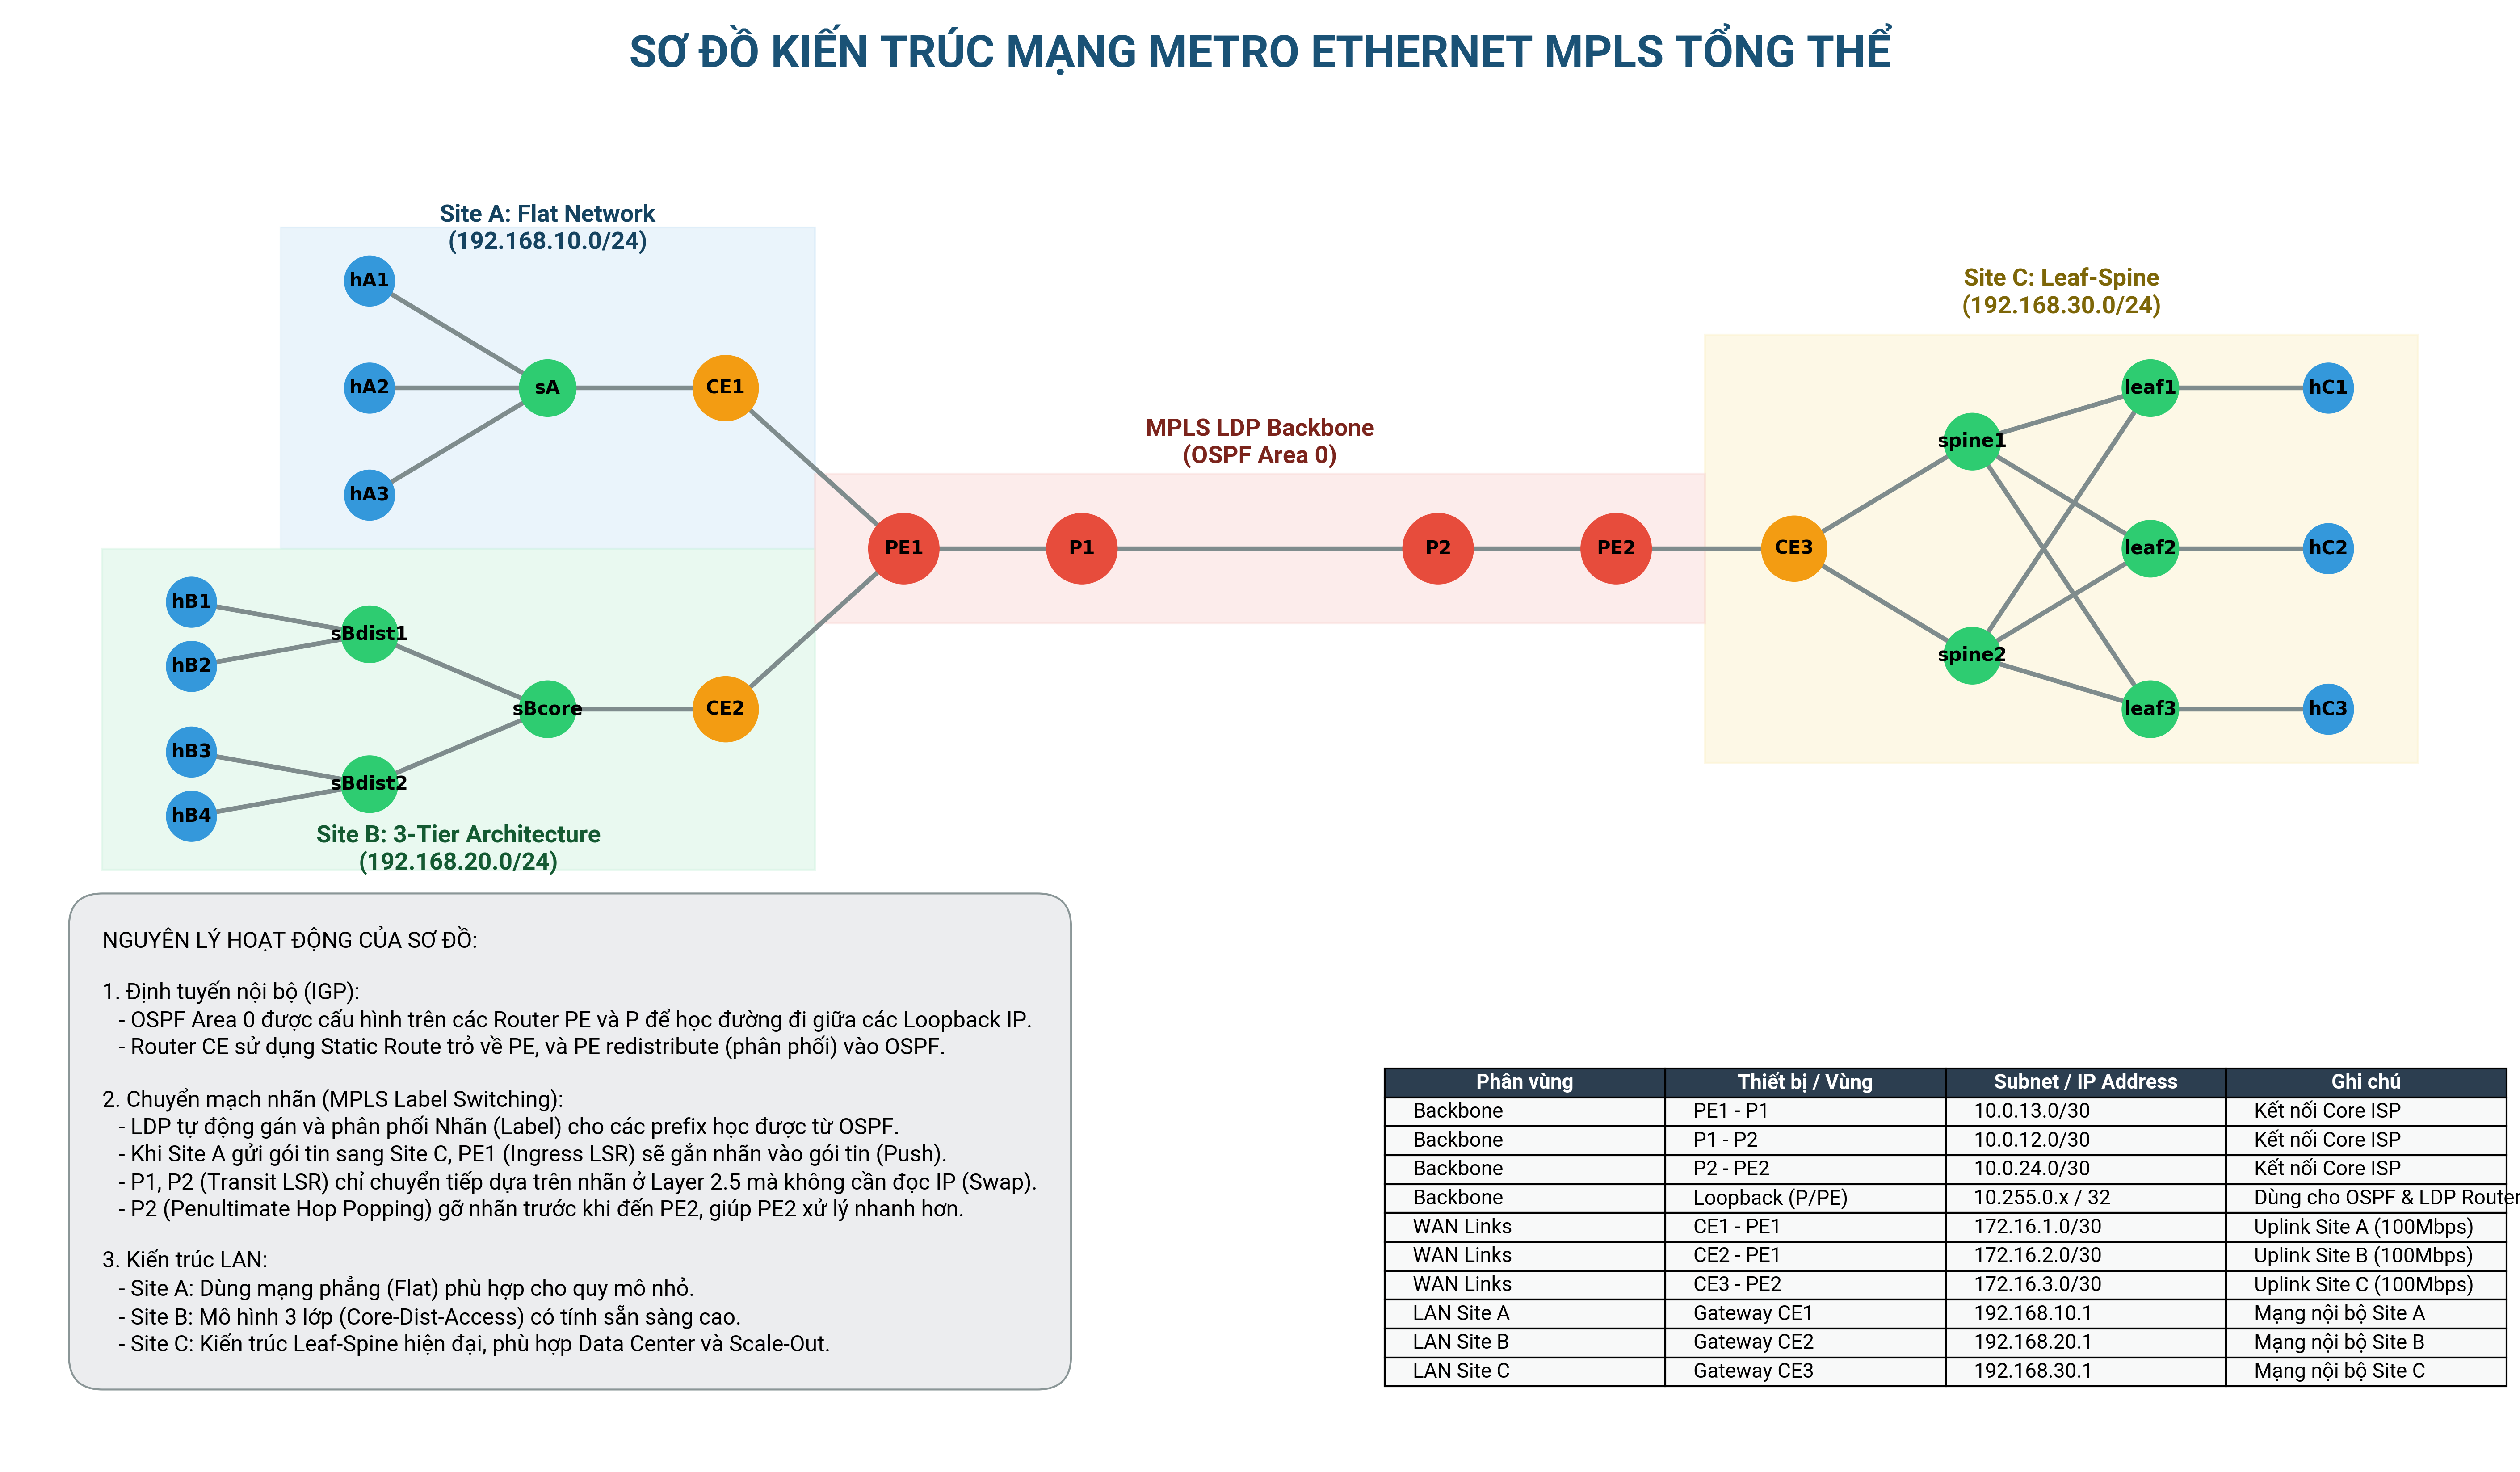
\includegraphics[width=0.9\textwidth]{image/network_topology.png}
    \caption{Sơ đồ kiến trúc mạng Metro Ethernet MPLS tổng thể}
    \label{fig:topology}
\end{figure}

\textit{\textbf{Giải thích minh chứng:}} Hình \ref{fig:topology} phác họa chi tiết thiết kế hệ thống. Trong đó, lõi mạng ISP được đặt ở giữa với các Router P1, P2 (Core) và PE1, PE2 (Edge). Ba mạng LAN nội bộ kết nối thẳng vào PE thông qua các Router biên khách hàng (CE1, CE2, CE3). Tuyến liên kết màu đỏ biểu diễn đường hầm MPLS ảo sẽ được thiết lập tự động bởi các giao thức định tuyến.

\subsection{Quy hoạch và Phân vai thiết bị}
Mô phỏng sử dụng tất cả 11 Switch, 7 Router và 10 Host, giả lập một mô hình có quy mô tầm trung thực tế.

\begin{table}[H]
    \centering
    \begin{tabular}{|p{3.5cm}|p{3.5cm}|p{7.5cm}|}
    \hline
    \rowcolor[HTML]{2C3E50} 
    \color{white} \textbf{Phân loại Nhóm} & \color{white} \textbf{Tên thiết bị} & \color{white} \textbf{Chức năng và Nhiệm vụ} \\ \hline
    \textbf{Core Router (P)} & P1, P2 & Đóng vai trò Router lõi xương sống của ISP. Không kết nối với khách hàng. Chuyên trách hoán đổi nhãn MPLS (Swap) để trung chuyển gói tin ở tốc độ tối đa. \\ \hline
    \textbf{Edge Router (PE)} & PE1, PE2 & Nằm ở biên mạng ISP. Có chức năng đóng/mở nhãn MPLS (Push/Pop) đối với các gói tin đi vào/đi ra từ mạng khách hàng. Định tuyến tĩnh để đón lưu lượng LAN. \\ \hline
    \textbf{Customer Router (CE)} & CE1, CE2, CE3 & Đặt tại trụ sở khách hàng. Đóng vai trò Gateway. Thiết lập đường tĩnh trỏ thẳng toàn bộ lưu lượng (Default Route) về phía nhà mạng (PE). \\ \hline
    \textbf{Site A (Mạng Flat)} & s1 & Switch Layer 2 thuần túy, mọi Host cắm chung vào mặt phẳng s1. Không có tính năng dự phòng. \\ \hline
    \textbf{Site B (Mạng 3-Tier)} & Core (s2), Dist (s3, s4), Access (s5, s6) & Thiết kế tam cấp. Đảm bảo nếu một Dist Switch sập, hệ thống vẫn duy trì hoạt động nhờ đường dự phòng vòng qua Dist Switch còn lại. \\ \hline
    \textbf{Site C (Leaf-Spine)} & Spine (s7, s8), Leaf (s9, s10, s11) & Thiết kế lưới toàn phần. Spine s7 và s8 đấu trực tiếp vào CE. Các Leaf nhận Host, tạo băng thông rộng lớn và độ trễ thấp (single-hop). \\ \hline
    \end{tabular}
    \caption{Phân quyền và chức năng chi tiết các thiết bị mạng}
    \label{tab:devices_planning}
\end{table}

\subsection{Quy hoạch không gian địa chỉ IP}
Dựa trên nguyên tắc tối ưu hóa bảng định tuyến, sơ đồ IP được phân mảnh khoa học. Các đường trục (Backbone) sử dụng Subnet mask /30 nhằm tiết kiệm tối đa dải IP Public. Không gian Private /24 được cấp phát cho các chi nhánh LAN để đáp ứng khoảng hơn 250 thiết bị mỗi vùng.

\begin{table}[H]
    \centering
    \begin{tabular}{|p{4.5cm}|>{\centering\arraybackslash}p{4cm}|p{6cm}|}
    \hline
    \rowcolor[HTML]{2C3E50} 
    \color{white} \textbf{Phân vùng mạng} & \color{white} \textbf{Subnet / IP Cụ thể} & \color{white} \textbf{Ghi chú / Cổng giao tiếp} \\ \hline
    \textbf{Loopback (OSPF ID)} & 10.255.0.x / 32 & Dành riêng cho P1(1), P2(2), PE1(3), PE2(4) \\ \hline
    \textbf{Backbone: P1 - PE1} & 10.0.13.0 / 30 & P1(.2), PE1(.1) - Nối giữa Core và Edge \\ \hline
    \textbf{Backbone: P2 - PE2} & 10.0.24.0 / 30 & P2(.2), PE2(.1) - Nối giữa Core và Edge \\ \hline
    \textbf{Backbone: P1 - P2}  & 10.0.12.0 / 30 & P1(.1), P2(.2) - Trục ngang xương sống lõi \\ \hline
    \textbf{WAN: PE1 - CE1}     & 172.16.1.0 / 30 & Kết nối chặng đầu tiên Site A ra ngoài \\ \hline
    \textbf{WAN: PE2 - CE2}     & 172.16.2.0 / 30 & Kết nối chặng đầu tiên Site B ra ngoài \\ \hline
    \textbf{WAN: PE2 - CE3}     & 172.16.3.0 / 30 & Kết nối chặng đầu tiên Site C ra ngoài \\ \hline
    \textbf{LAN Site A (Flat)}  & 192.168.10.0 / 24 & Gateway CE1 (.1). Client (.11 đến .13) \\ \hline
    \textbf{LAN Site B (3-Tier)}& 192.168.20.0 / 24 & Gateway CE2 (.1). Client (.11 đến .14) \\ \hline
    \textbf{LAN Site C (Spine)} & 192.168.30.0 / 24 & Gateway CE3 (.1). Client (.11 đến .13) \\ \hline
    \end{tabular}
    \caption{Chi tiết quy hoạch và phân bổ vùng địa chỉ IP}
    \label{tab:ip_planning}
\end{table}

\subsection{Chiến lược Định tuyến và Phân phối nhãn MPLS}

Để toàn bộ các máy tính từ 3 chi nhánh nhìn thấy nhau, chiến lược định tuyến được thiết kế như sau:

\paragraph{1. Định tuyến biên (CE - PE): Định tuyến tĩnh tối giản}
Do Router CE của khách hàng là thiết bị nhỏ gọn (Customer Premises Equipment), chúng ta không chạy định tuyến động tốn tài nguyên. Tại CE1, CE2, CE3 chỉ cần thiết lập duy nhất một Default Route (0.0.0.0/0) đẩy toàn bộ lưu lượng về PE tương ứng.
Tại PE1 và PE2, nhà mạng sẽ cấu hình Static Route chỉ đích danh Subnet của khách hàng trỏ ngược lại CE. 

\paragraph{2. Định tuyến Lõi (Core OSPF Area 0)}
Tại 4 Router lõi P1, P2, PE1, PE2, giao thức OSPF Area 0 được kích hoạt. OSPF sẽ lắng nghe trên các cổng Backbone (dải 10.0.x.x) và tự động học các địa chỉ Loopback (10.255.0.x) của nhau. Thông qua thao tác \textit{Redistribute Static}, các PE router sẽ chèn thông tin dải mạng LAN (192.168.x.0/24) của khách hàng vào bảng OSPF, chia sẻ cho phần còn lại của mạng lưới.

\paragraph{3. Hoạt động Chuyển mạch nhãn LDP (MPLS Data Plane)}
Sự kỳ diệu của mạng nằm ở tầng LDP:
\begin{itemize}
    \item LDP được kích hoạt trên tất cả giao diện nối giữa P và PE.
    \item Dựa trên bảng định tuyến OSPF đã hoàn chỉnh, LDP tự động tạo ra một Nhãn (Label) cho mỗi dải IP đích, và gửi nhãn này báo cho các láng giềng.
    \item Khi gói tin từ chi nhánh A đi sang chi nhánh C: Tại cửa ngõ vào (PE1), gói tin bị đóng thêm nhãn (Push Label). Đến giữa đường (P1, P2), các router chỉ đọc nhãn, đổi nhãn khác (Swap) và ném đi chứ không phải mổ xẻ IP.
    \item Gần đến đích (P2), router chủ động tháo nhãn (Pop) nhờ cơ chế Penultimate Hop Popping (PHP) trước khi giao cho PE2, để PE2 đỡ tốn công xử lý, giúp gói tin đến Site C nhanh nhất có thể.

\subsection{Minh chứng sơ bộ việc khởi tạo đúng Topology đề tài}
Để khẳng định mô hình đã được xây dựng đúng chuẩn với những thiết kế lý thuyết ở trên, ngay sau khi khởi động hệ thống giả lập Mininet, ta sẽ kiểm tra toàn bộ danh sách các Node và các Link (đường truyền) kết nối giữa chúng.

\begin{figure}[H]
    \centering
    % [NOTE] TRONG TERMINAL MININET, GÕ LỆNH `nodes` VÀ `net`. CHỤP ẢNH MÀN HÌNH CHỨA KẾT QUẢ CỦA 2 LỆNH NÀY VÀ LƯU VÀO FOLDER image/ TÊN LÀ mininet_nodes_net.png
    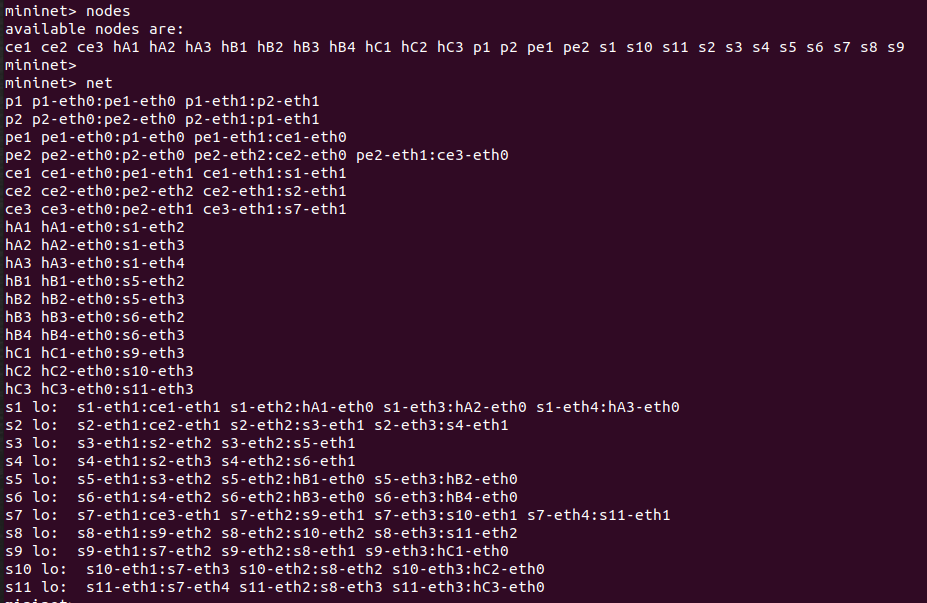
\includegraphics[width=0.8\textwidth]{image/mininet_nodes_net.png}
    \caption{Danh sách thiết bị (Nodes) và Liên kết mạng (Net) trên Mininet}
    \label{fig:mininet_nodes}
\end{figure}

\textit{\textbf{Giải thích minh chứng:}} Từ kết quả lệnh \texttt{nodes} và \texttt{net}, ta thấy rõ hệ thống đã khởi tạo đủ 17 Hosts (bao gồm các Router P1, P2, PE1, PE2, CE1, CE2, CE3 và các máy trạm hA1-hA3, hB1-hB4, hC1-hC3) cùng với 11 Switch mạng (từ s1 đến s11). Lệnh \texttt{net} minh họa chính xác các cáp nối vật lý ảo giữa chúng, đảm bảo cấu trúc Topology được thiết lập một cách hoàn hảo:
\begin{itemize}
    \item Site A kết nối qua Switch phẳng \texttt{s1} (với hA1, hA2, hA3).
    \item Site B nối phân cấp 3 lớp chuẩn mực từ Router CE2 xuống Core \texttt{s2}, rẽ nhánh sang Distribution \texttt{s3, s4} và đổ xuống Access \texttt{s5, s6} chứa các máy trạm hB.
    \item Và đặc biệt nhất là Site C được đấu chéo dạng lưới Full-Mesh giữa các Spine (\texttt{s7, s8}) và các Leaf (\texttt{s9, s10, s11}) đúng với lý thuyết đã trình bày (có thể thấy rõ các đường nối như \texttt{s7-eth2:s9-eth1}, \texttt{s8-eth1:s9-eth2}).
\end{itemize}

Sau khi đảm bảo thiết bị đã đầy đủ, ta tiến hành gửi gói tin ICMP (Ping) liên tục từ Site A đến Site B và Site C để chứng minh toàn mạng thông suốt:

\begin{figure}[H]
    \centering
    % [NOTE] TRONG TERMINAL MININET, GÕ LỆNH `hA1 ping -c 8 192.168.20.11` VÀ `hA1 ping -c 8 192.168.30.11` (Chờ mạng hội tụ 35 giây trước khi gõ). CHỤP MÀN HÌNH 2 KẾT QUẢ NÀY (ĐẠT 0% LOSS) LƯU VÀO image/ TÊN LÀ ping_toan_mang.png
    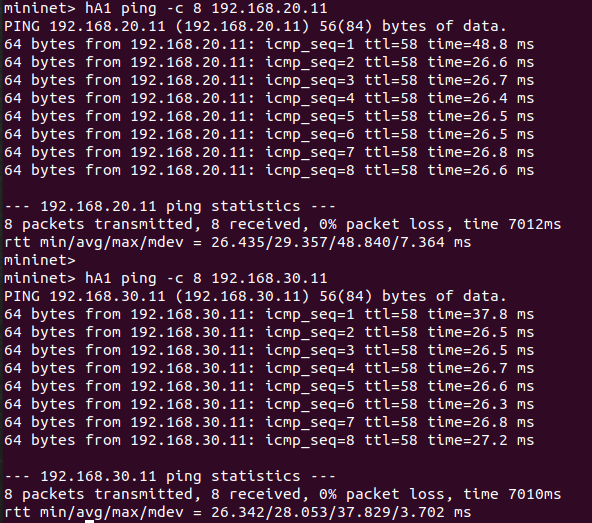
\includegraphics[width=0.8\textwidth]{image/ping_toan_mang.png}
    \caption{Kiểm tra thông mạch toàn mạng bằng 8 gói tin Ping}
    \label{fig:ping_toan_mang}
\end{figure}

\textit{\textbf{Giải thích minh chứng:}} Lệnh Ping với tham số \texttt{-c 8} ép hệ thống gửi liên tục 8 gói tin giữa các chi nhánh ở xa nhau. Ở kết quả trả về thực tế, gói tin đi từ hA1 (Site A) sang hB1 (Site B - IP 192.168.20.11) và từ hA1 sang hC1 (Site C - IP 192.168.30.11) đều nhận được \textbf{8 phản hồi (8 received)} và cho ra \textbf{0\% packet loss}. Độ trễ (RTT) trung bình duy trì cực kỳ ổn định ở mức \textbf{29.357 ms} (cho hướng Site B) và \textbf{28.053 ms} (cho hướng Site C). Đây là bằng chứng thép cho thấy toàn bộ kiến trúc 3 mô hình LAN và mạng lõi MPLS Backbone đã được cấu hình thành công, không hề xảy ra nghẽn mạng hay vòng lặp định tuyến. Mọi chi nhánh đều có thể giao tiếp với nhau trơn tru như một mạng nội bộ duy nhất.
